\addplot+[mark=square*] coordinates {(1,.964)(2,.950)(3,.958)(4,.928)(5,.707)(6,.603)(7,.923)(8,.860)};
\legend{Authenticated success,Mean label accuracy}
\end{axis}
\end{tikzpicture}
\caption{Holdout robustness at message and pre-FEC label levels. G denotes Gaussian noise, B blur, C crop percentage, and R rotation degrees. The gap between label accuracy and authenticated recovery visualizes protection supplied by majority grouping and RS128.}
\Description{Line chart comparing authenticated success and mean pre-FEC label accuracy for eight holdout transformations. Seven transformations have perfect message success; the 12 percent crop has 113 of 150 successes.}
\label{fig:holdout}
\end{figure}

\begin{figure}[t]
\centering
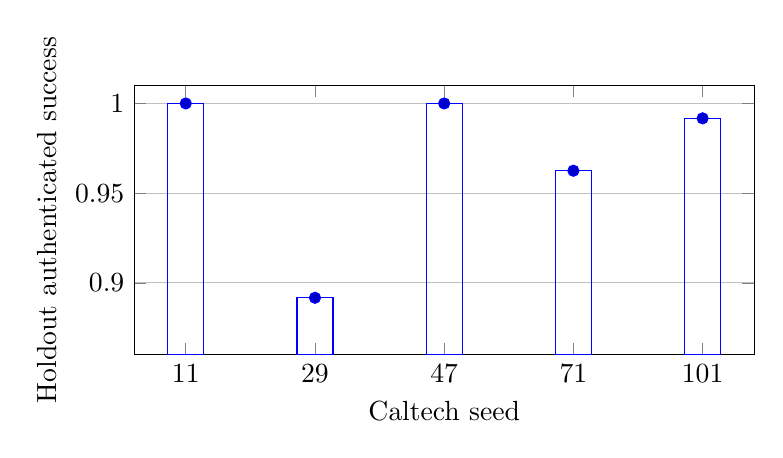
\begin{tikzpicture}
\begin{axis}[width=.78\textwidth,height=5cm,ymin=.86,ymax=1.01,xtick={1,2,3,4,5},xticklabels={11,29,47,71,101},xlabel={Caltech seed},ylabel={Holdout authenticated success},ymajorgrids=true]
\addplot+[ybar,bar width=13pt] coordinates {(1,1)(2,.8917)(3,1)(4,.9625)(5,.9917)};
\end{axis}
\end{tikzpicture}
\caption{External holdout authenticated-message success by partition. The aggregate across all five partitions is 96.92\%.}
\Description{Bar chart showing holdout authenticated-message success by seed: 1.0, approximately 0.892, 1.0, 0.963, and 0.992.}
\label{fig:holdoutseed}
\end{figure}

\subsection{RS-parity ablation and communication cost}
The controlled parity ablation shows that RS coding materially changes authenticated holdout recovery. With no RS parity, group-majority decoding alone recovers 829/1,200 trials (69.08\%). Recovery rises to 1,064/1,200 (88.67\%) at RS32, 1,115/1,200 (92.92\%) at RS64, 1,145/1,200 (95.42\%) at RS96, and 1,163/1,200 (96.92\%) at RS128. Mean transmitted images per session rise from 970 without parity to 1,396.7, 1,825, 2,250, and 2,676.7. At RS128, 8-, 32-, and 64-byte plaintexts require 2,320, 2,640, and 3,070 transmitted images, corresponding to 0.0276, 0.0970, and 0.1668 useful bits per transmitted image.
\begin{table}[t]
\caption{Controlled external RS-parity ablation.}
\label{tab:rsablation}
\small
\begin{tabular}{rrrr}
\toprule
Parity bytes & Auth. recovery & Success & Mean images/session\\
\midrule
0&829/1,200&69.08\%&970.0\\
32&1,064/1,200&88.67\%&1,396.7\\
64&1,115/1,200&92.92\%&1,825.0\\
96&1,145/1,200&95.42\%&2,250.0\\
128&1,163/1,200&96.92\%&2,676.7\\
\bottomrule
\end{tabular}
\end{table}
\begin{table}[t]
\caption{Implemented RS128 communication cost by plaintext size.}
\label{tab:commcost}
\small
\begin{tabular}{rrrr}
\toprule
Plaintext & Coded groups & Images sent & Net bits/image\\
\midrule
8 B&464&2,320&0.0276\\
32 B&528&2,640&0.0970\\
64 B&614&3,070&0.1668\\
\bottomrule
\end{tabular}
\end{table}
\begin{figure}[t]
\centering
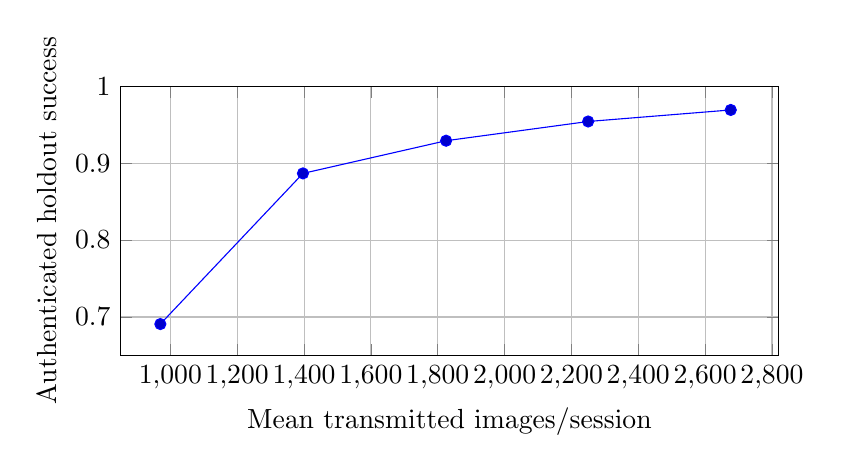
\begin{tikzpicture}
\begin{axis}[width=.82\textwidth,height=5cm,xmin=850,xmax=2820,ymin=.65,ymax=1.0,xlabel={Mean transmitted images/session},ylabel={Authenticated holdout success},ymajorgrids=true,xmajorgrids=true]
\addplot+[mark=*] coordinates {(970,.6908)(1396.7,.8867)(1825,.9292)(2250,.9542)(2676.7,.9692)};
\end{axis}
\end{tikzpicture}
\caption{Measured reliability--communication tradeoff in the frozen external parity ablation.}
\Description{Line plot showing authenticated holdout success increasing from 0.6908 at 970 transmitted images per session with RS0 to 0.9692 at 2676.7 images with RS128.}
\label{fig:rstradeoff}
\end{figure}

\subsection{Selection detectability}
Table~\ref{tab:detectors} summarizes the final detector audit. SRM-lite remains close to chance, GLCM reveals a small repeatable texture/selection shift, and the trained CNN provides the strongest discrimination with mean macro-AUC 0.5266. The five CNN seed means lie between 0.5232 and 0.5301, showing that the signal persists across external partitions. The supported characterization is therefore low but measurable selection leakage under the evaluated matched-index warden.

\begin{table}[t]
\caption{Final repeated Caltech-101 selection-detector audit ($n=100$ overlapping image-disjoint splits per detector). Intervals summarize repeated-split variability.}
\label{tab:detectors}
\small
\begin{tabular}{lrrrr}
\toprule
Detector & Mean AUC & SD & Min--Max & Descriptive 95\% interval\\
\midrule
SRM-lite + ExtraTrees&0.5040&0.0023&0.4969--0.5088&0.5036--0.5045\\
GLCM + logistic&0.5128&0.0017&0.5088--0.5162&0.5125--0.5132\\
30-head CNN&0.5266&0.0034&0.5186--0.5340&0.5259--0.5273\\
\bottomrule
\end{tabular}
\end{table}

\begin{figure}[t]
\centering
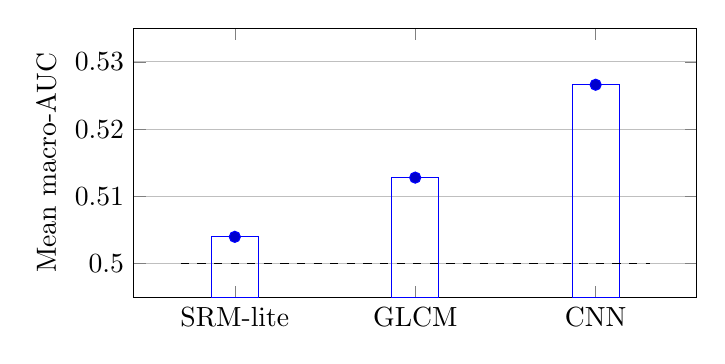
\begin{tikzpicture}
\begin{axis}[width=.72\textwidth,height=5cm,ymin=.495,ymax=.535,xtick={1,2,3},xticklabels={SRM-lite,GLCM,CNN},ylabel={Mean macro-AUC},ymajorgrids=true]
\addplot+[ybar,bar width=17pt] coordinates {(1,.5040)(2,.5128)(3,.5266)};
\addplot[domain=.7:3.3,dashed] {.5};
\end{axis}
\end{tikzpicture}
\caption{Mean macro-AUC of the frozen detector battery. The dashed reference is chance AUC 0.5.}
\Description{Three-bar chart with mean AUC 0.504 for SRM-lite, 0.513 for GLCM, and 0.527 for CNN; a dashed line marks chance at 0.5.}
\label{fig:detectors}
\end{figure}

The CNN evidence comprises 20/20 successful workflow jobs, 100 repetition-level macro-AUC rows, and 3,000 per-session-head AUC rows. This granularity supports both aggregate and partition-level inspection of learned detector behavior.
